\chapter{Experimental Setup and Sample Systems} \label{ch_exp}

\section{Synchrotron Radiation}
The radiation emitted by a relativistic charged particle, usually electrons, accelerated to a circular orbit through an external magnetic field is called synchrotron radiation. This radiation is polarized and emitted tangentially to the circular movement of the charged particle in forward direction. In the history of synchrotron radiation, sources have evolved from parasitic use of particle accelerators to the extend of building electron storage rings dedicated for the sole purpose of generating this radiation \cite{munro_chapter_1987}. Its most promitent features are the high brilliance, that is the number of photons per second per unit particle beam cross section and per unit solid angle within $0.1\%$ bandwidth at a specific wavelength, and its huge spectral range of emission. Depending on the energy of the relativistic particles forced on a circular orbit, in modern electron storage rings typically in the order of one to several GeV, the emission covers the range from the terahertz into the hard X-ray regime. The \gls{ptb} operates two laboratories at the dedicated sources, the \gls{bessy} and the \gls{mls} \cite{brandt_metrology_2007}. The two thrid-generation synchrotron radiation sources provide maximum electron energies of $1.7$ GeV (\gls{bessy}) and $0.6$ GeV (\gls{mls}), respectively. Theoretical emission spectra for a single dipole magnet (\emph{bending magnet}) are shown in Fig.~\ref{ch_exp:fig_experimental_synchrotron_spectra} in comparison to black body radiation.
\begin{figure}
 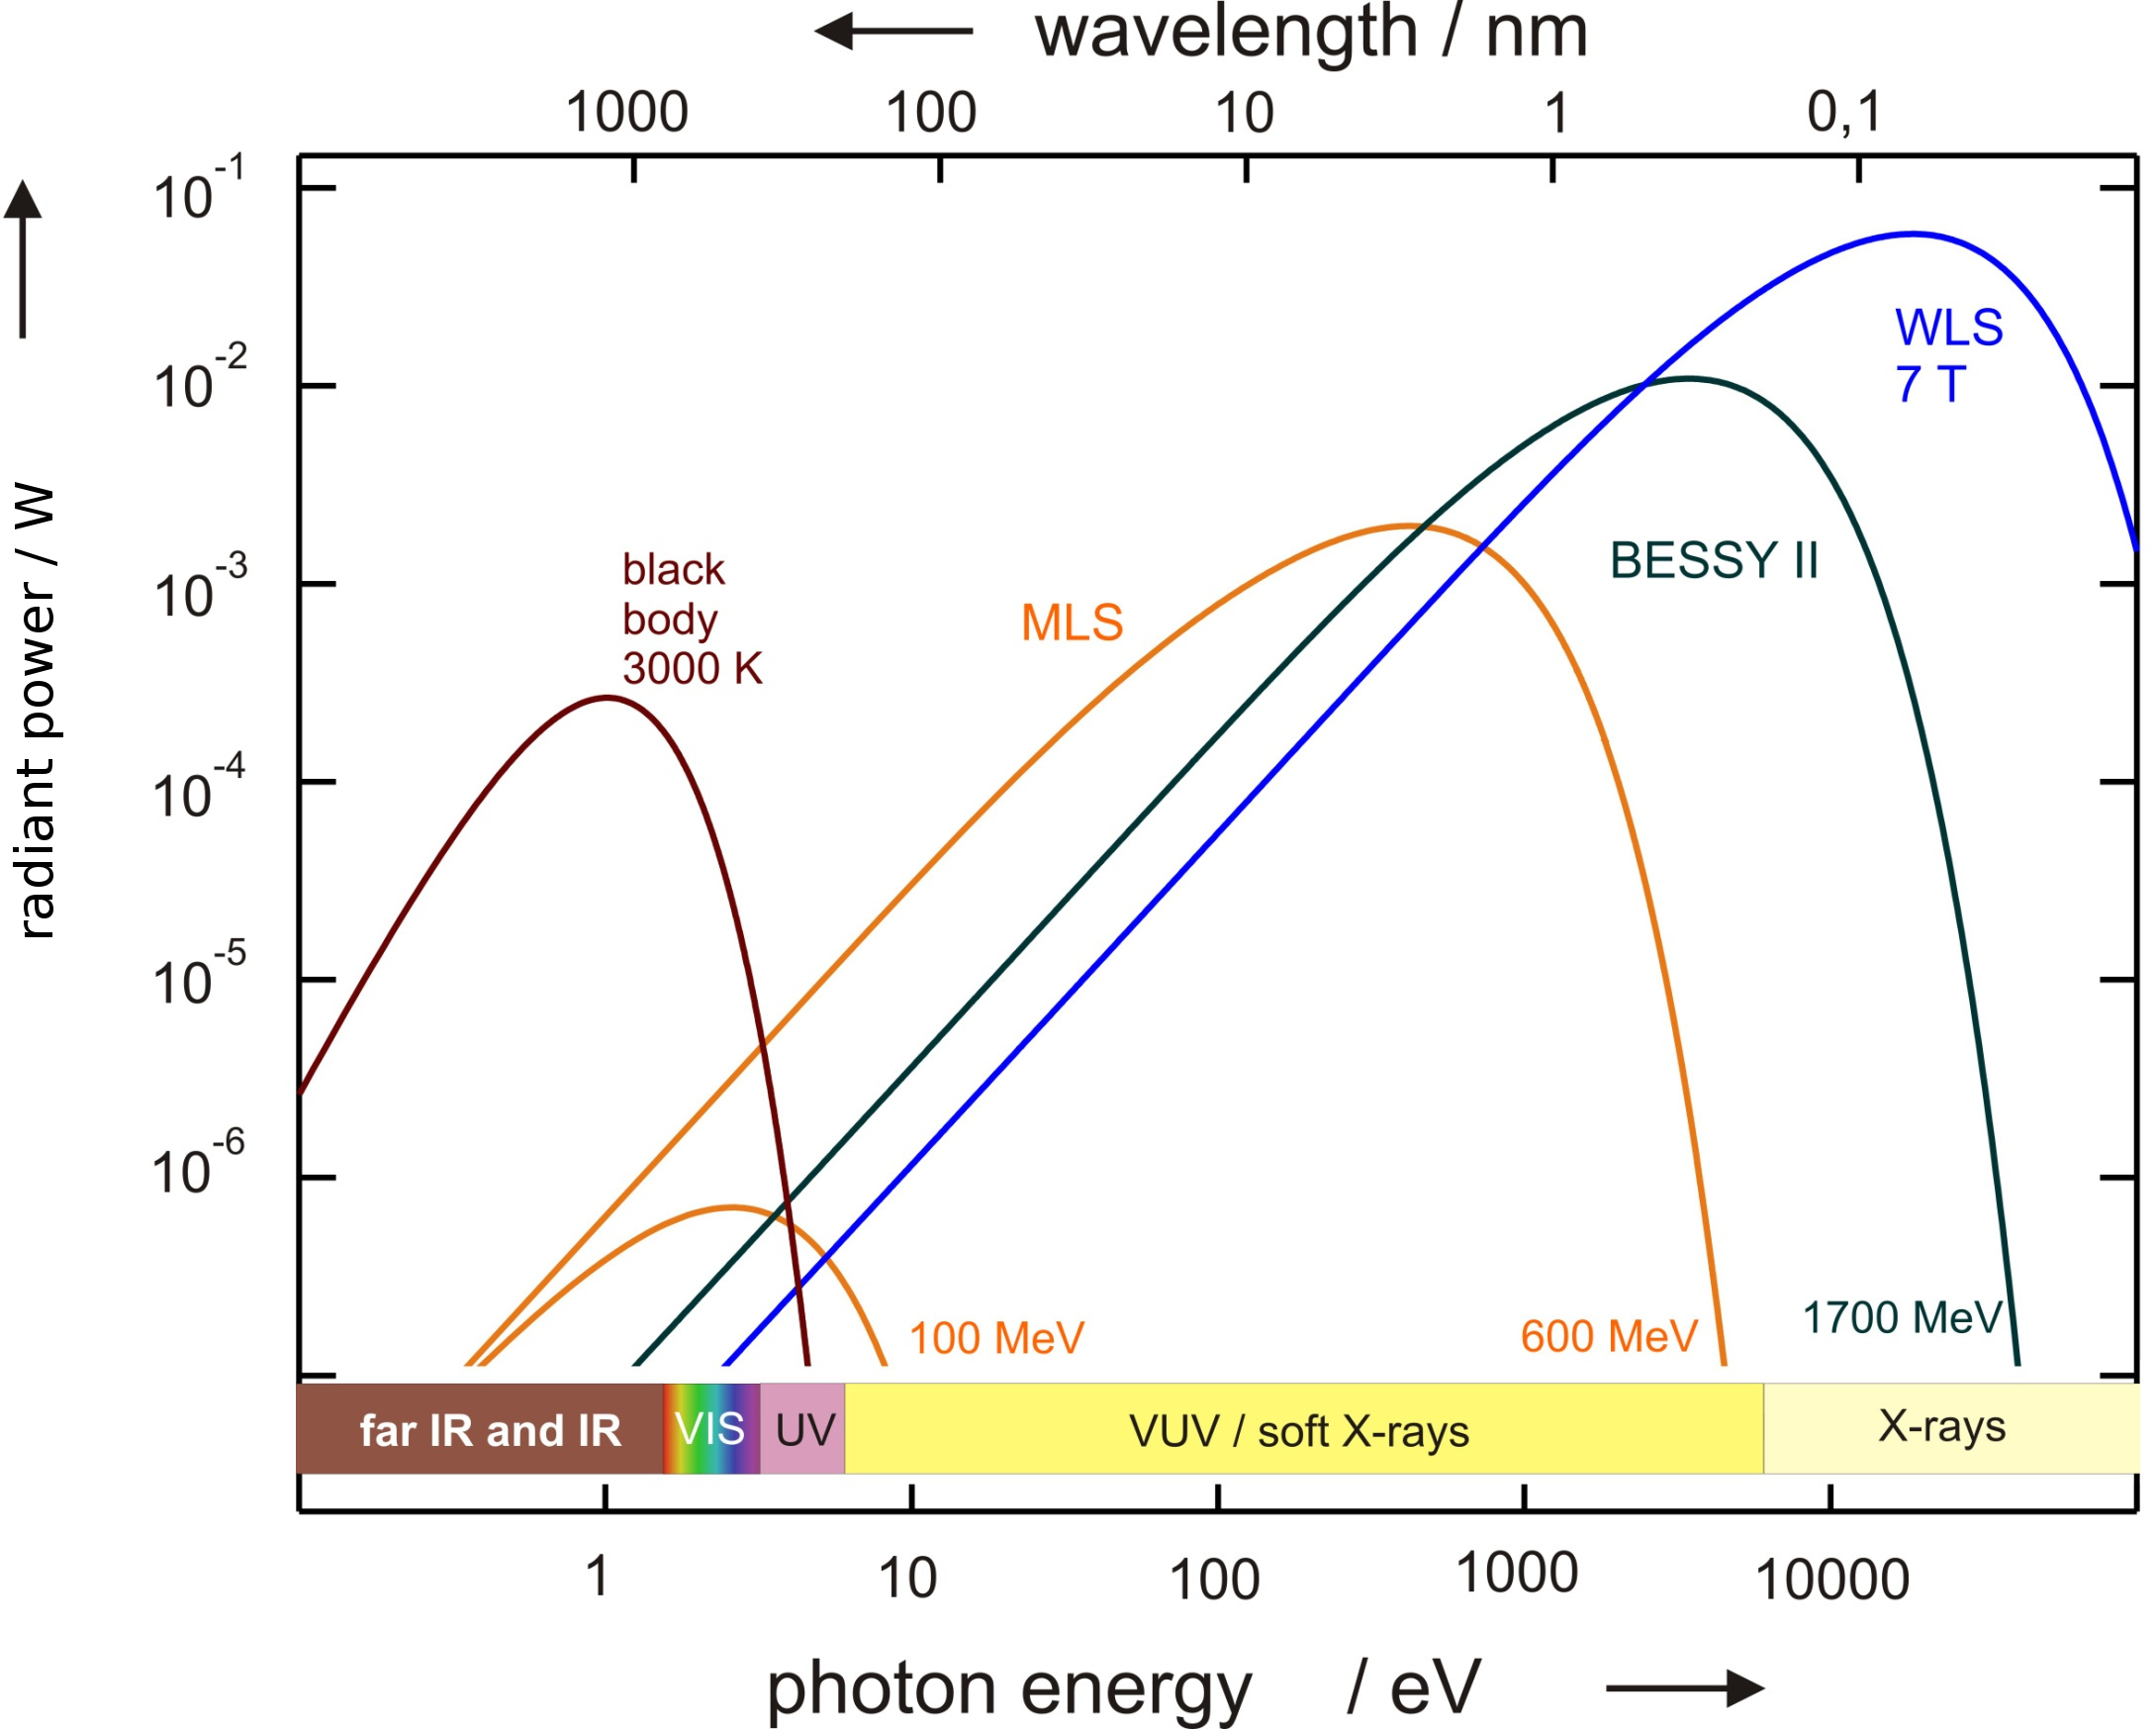
\includegraphics[width=0.7\textwidth]{img/exp-bessy-dipole-spectrum.jpeg}
 \caption[Theoretical synchrotron radiation radiant power spectra]{Theoretical synchrotron radiation radiant power spectra for the \gls{mls} and \gls{bessy} in comparison to black body radiation\footnote{Image taken from \textcite{beckhoff_quarter-century_2009}}. The curves show the radiant power of emission for bending magnets at both electron storage ring facilities for different electron energies. The curve marked WLS shows the radiant power from the $7$ Tesla wavelength shifter insertion device installed at \gls{bessy}.}
 \label{ch_exp:fig_experimental_synchrotron_spectra}
\end{figure}

A very important theoretical aspect of synchrotron radiation, apart from the high brilliance and large spectrum, is the fact that the emission can be calculated exactly from first principles of classical electrodynamics and special relativity. The theory for synchrotron radiation was developed by Schwinger \cite{schwinger_classical_1949} and we shall review its most imporant aspects here. Given all the fundamental and experimental parameters are known, the total emitted radiant power per relativistic particle can be calculated exactly as
\begin{align}
 P = \frac{1}{4 \pi \gls{epsilon_0}} \frac{2}{3} \frac{\gls{e}^2 \gls{c}}{R^2}\Big( \frac{E}{\gls{m_0} \gls{c}^2}\Big)^4 \text{,} \label{ch_exp:schwinger_equation_total_power}
\end{align}
where \gls{e} is the elementary charge, \gls{c} is the speed of light in vacuum, $E$ is the particles energy, \gls{m_0} is the rest mass of the particle and $R$ is the radius of the circular trajectory imposed by the magnetic field. The radiant power is thus inversely proportional to the fourth power of the particles rest mass, which explains the usage of light electrons in comparison with significanlty heavier protons in synchrotron radiation sources. The dependence on the electron energy is visible in another characteristic value for the emitted radiant power, visible as a shift to higher photon energies (smaller wavelengths) in Fig.~\ref{ch_exp:fig_experimental_synchrotron_spectra}, known as the critical energy or critical wavelength \cite{schwinger_classical_1949}, respectively,
\begin{align}
 E_C = \frac{3 \gls{h} \gls{c}}{4 \pi R} \Big( \frac{E}{\gls{m_0} \gls{c}^2}\Big)^3 \text{.} \label{ch_exp:characteristic_energy}
\end{align}
It marks the point in the spectrum, where the integrated radiant power for all values above and below the critical energy are equal \cite{balerna_introduction_2015}. This formula quantifies the shift towards higher energies due to the increase of the electron energy comparing the \gls{mls} and \gls{bessy} emission spectra. Apart from the spectral distribution, the emitted radiation is linearly polarized with an electric field vector oscillating parallel to the plane of the circular orbit. This property, however, is only stricly valid for the emission inside this plane. For radiation above or below, a vertical polarization component (parallel to the surface normal of the orbital plane) exsists. The intensity $I(\lambda,\Psi)$ emitted by a single electron on a circular orbit in direction of the azimuthal angle $\Psi$ at the wavelength $\lambda$ is described by
\begin{align}
  I(\lambda,\Psi) &= \frac{27 \gls{e}^2 \gamma^8 }{36 \pi^3 R^3} \Big(\frac{\lambda_c}{\lambda}\Big)^4 \big(1+ (\gamma \Psi)^2\big)\Big( K_{2/3}^2(\zeta) + \frac{(\gamma \Psi)^2}{1 + (\gamma \Psi)^2} K_{1/3}^2(\zeta)\Big) \text{,}
 \label{ch_exp:schwinger_equation_spectral}
\end{align}
where $\gamma = \sfrac{E}{\gls{m_0} \gls{c}^2}$ and $\Psi$ is the angle between the orbital plane and the observation direction outside of that plane \cite{schwinger_classical_1949}. The characteristic wavelength $\lambda_c = \sfrac{h c}{E_c}$ is given by the critical photon energy defined in Eq.~\eqref{ch_exp:characteristic_energy}. The argument of the modified Bessel funktions of second kind $K_{x}(\zeta)$ is defined as
\begin{align}
 \zeta = \frac{\lambda}{\lambda_c} \big(1 + (\gamma \Psi)^2\big)^\frac{3}{2} \text{.}
\end{align}


The ability to calculate the exact emission and polarization properties of synchrotron radiation based on Eq.~\eqref{ch_exp:schwinger_equation_spectral} with a given electron current and aceptance angle have another very valuable side effect for the field of metrology. It enables the use of synchrotron radiation as a primary standard for electromagnetic radiation within the available spectral range, which is in fact exploited by the \gls{ptb} \cite{thornagel_electron_2001} to provide absolute radiometry.

The dedicated sychrotron radiation facilities, such as \gls{bessy} and the \gls{mls} provide additional possibilities of generating synchrotron radiation beyond a simple bending magnet through different instertion devices. Fig.~\ref{ch_exp:fig_bessy2} gives a shematic overview over the storage ring \gls{bessy}. At each of the marked dipole magnets, synchrotron radiation is produced according the theory presented above. The radiation is transmitted through outlet systems towards a large number of beamlines, which monochromatize and focus the radiation for experimental applications.
\begin{figure*}[htb]
    \def\svgwidth{0.7\textwidth}
    \import{svg/}{bessy.pdf_tex}
    \caption[Schematic overview of BESSY II.]{Schematic overview of the electron storage ring facility \gls{bessy}\footnote{Original image by \gls{hzb}, Ela Strickert, source: \url{https://www.helmholtz-berlin.de/mediathek/bildarchiv/}}. The synchrotron accelerates the electrons coming from the \gls{linac}, which are then injected in the electron storage ring with their full desired energy. Electromagnetic lenses focus and stabilize the beam, as well as deflecting it onto the circular orbit while emitting synchrotron radiation at each dipole (bending) magnet. Cavities reaccelerate the electrons in the storage ring to compensate the energy loss due to the radiation emission.}
    \label{ch_exp:fig_bessy2}
\end{figure*}
Undulators or wigglers are inserted in the straight sections of the \gls{bessy} storage ring with a large number of periodically arranged magnets with alternating polarization forcing the electrons on a sinosoidal beam path. The goal of these insertion devices is to shift the critical energy of the storage ring towards higher energies (wigglers) or to dramatically increase the brilliance within a significantly smaller spectral range compared to bending magnets (undulators). The different effect of the undulators and wigglers on the generated spectrum is determined by the magnetic field strength $B_0$ and the distance between two identical periodic arragnements of the magnets of alternating polarization $\lambda_0$. The deflection parameter quantifies this relation through $K \propto B_0 \lambda_0$. Undulators typically have deflection parameters $K < 1$ while in case of wigglers $K \gg 1$ \cite{munro_chapter_1987}. Technically, the magnetic field strength can be varied by changing the distance (``gap'') between the magnets vertically. By changing the vertical alignment of the magnetic field direction with respect to the beam path, it is even possible to affect the polarization properties of the emitted radiation to obtain circularly or eliptically polarized radiation.
\begin{figure}[htb]
    \def\svgwidth{0.7\textwidth}
    \import{svg/}{mls.pdf_tex}
    \caption[Schematic overview of the MLS]{Schematic overview of the electron storage ring facility \gls{mls}}
    \label{ch_exp:fig_mls}
\end{figure}


The most advanced light source available today, also known as fourth generation source, is following the concept of a \gls{fel} as first invented by \textcite{madey_stimulated_1971}. In that case radiation is produced by a typically single very long undulator inside a linear accelerator instead of a comparatively short straight section of a storage ring. The concept was first demonstrated by \textcite{deacon_first_1977}. \Gls{fel} sources produce highly coherent radiation in the x-ray regime through the principle of \gls{sase} \cite{derbenev_possibility_1982, bonifacio_collective_1984}. Here, the emitted radiation inside the long undulator has a feedback effect on the electron bunch travelling along the beam path. The result is a microbunching of the electron cloud through the electric field of the emitted radiation connected with a (random) wavelength within a certain spectral range defined by the undulator properties. The microbunching causes amplification of that wavelength, which causes an emission spectrum showing several spikes of amplified wavelengths with a noisy background until a saturation level is reached \cite{milton_exponential_2001}.

\section{The Instrumentation for the EUV Spectral Range}
\subsection{The EUV Beamlines at BESSYII and MLS}
The radiation generated in bending magnets or in insertion devices in synchrotron radiation sources typically requires monochromatization and focussing trough a series of optical elements depending on the experimental requirements or designated use cases. In addition, radiation in the \gls{euv} spectral range is absorbed quickly during propagation under atmospheric conditions. It is thus neccessary to maintain a high vacuum from the source points to the experiment and the detector. The two \gls{ptb} beamlines for the \gls{euv} spectral range at the two storage rings \gls{bessy} and \gls{mls} operate on the broad spectrum emitted by bending magnets at each facility. The experiments conducted in the framework of this thesis were performed at both beamlines, exploiting the different radiant power in the required spectral range of the respective experiments. The two beamlines share many technical and design aspects. Thus, the description here will introduce most of these aspects with respect to the SX700 beamline at \gls{bessy}. The differences of the \gls{euvr} at the \gls{mls} will be given below.

\subsubsection{The Soft X-ray Beamline SX700}
The \gls{sx700} at \gls{bessy} provides a monochromatic beam in the spectral range from $\nm{0.7}$ to $\nm{24.8}$ wavelength (corresponding to photon energy range from $\ev{50}$ to $\ev{1800}$) \cite{beckhoff_quarter-century_2009}. The total radiation power and the corresponding relative bandwidth at that beamline are shown in Fig.~\ref{ch_exp:fig_flux_sx700}. The beam size at the entrance aperture to the reflectometer (experimantal end station) is variable through the setting of the exit slits. In the standard setting is approximately \mm{1} by \mm{1} \cite{scholze_high-accuracy_2001} and can be reduced to \mm{0.1} vertical extent (grating dispersion direction) and \mm{0.5} horizontal extent.
\begin{figure}[htb]
    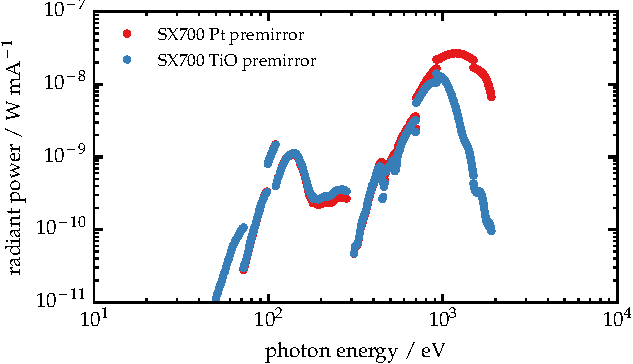
\includegraphics{img/beamline_radiant_power.pdf}
    \caption[Radiant power of the SX700 beamline.]{Radiant power of the SX700 beamline at \gls{bessy} in W per mA storage ring ring current. The two curves differ by the coating on the premirror in the beamline. The TiO coating provides the ability to achieve energies down to \ev{50}, while the Pt coating ensures high radiant power in the high energy range up to \ev{1800}.}
    \label{ch_exp:fig_flux_sx700}
\end{figure}

The monochromatization of the radiation is achieved by a plane grating monochromator with a blazed line grating with 1200 lines per millimeter mounted with its rotational axis within the plane of the storage ring and illuminated perpendicular to the grating lines, yielding the dispersive direction being perpendicular to the storage ring plane. The schematic layout of the beamline is illustrated in Fig.~\ref{ch_exp:fig_sx700_schematic} including the plane grating position of the monochromator, the focussing mirrors and slit positions.
\begin{figure*}[htb]
    \def\svgwidth{\textwidth}
    \import{svg/}{sx700_scheme.pdf_tex}
    \caption[Schematic setup of the SX700 beamline.]{Schematic setup of the \gls{sx700} beamline at \gls{bessy} in top view (upper part) and side view (lower part) \footnote{Original image taken from \textcite{scholze_high-accuracy_2001}}.}
    \label{ch_exp:fig_sx700_schematic}
\end{figure*}
The selection of the desired wavelength at the position of the experimental chamber is done by a horizontal slit at the exit slit. The achievable relative bandwidth depends on the size of this slit as well as on the selected wavelength. It varies between values of $0.5\times 10^{-3}$ and $2.5\times 10^{-3}$ relative bandwidth. As mentioned above, the monochromator grating disperses the incoming broad band radiation into the vertical direction with respect to the storage ring plane. The blaze of the grating ensures high grating efficiency of about $X \%$ in the first diffraction order, but the selected vertical part of the dispersed radiation still contains parts of higher diffraction orders. This leads to a diminished spectral purity, which reduces the energy resolution. For the purpose of suppression of these higher grating orders, thin metal films in transmission geometry acting as filters are installed close to the entrance aperture to the experimental station supressing radiation energetically above the respective absorption edges of the material.

The \gls{sx700} beamline only has one focussing mirror per horizontal and vertical direction, which differs in position in the beamline and produces different focal points for the two directions. The focussing in horizontal direction (grating dispersion direction) is done trough the toroidal mirror (cf.~Fig.~\ref{ch_exp:fig_sx700_schematic}), which also serves as a collector mirror for both axis and parallizes the beam in vertical direction. The focal point is located in the exit slit to ensure high energy resolution. The vertical focussing is done by an additional focussing mirror after the monochromator grating with a focal point about \m{2} behind the exit slit in propagation direction. Due to the large distance of the two focussing elements to the experimental station, a low divergence of the beam of about $1.6$ mrad $\times$ $0.4$ mrad is achieved.

\subsubsection{The Extreme Ultraviolet Beamline EUVR}
The general layout and operation principle of the \gls{euvr} beamline is identical to that of the \gls{sx700} beamline described in the previous paragraph with some differences in the focussing, which are described in the following. Due to the lower electron energy in the \gls{mls} storage ring, the spectrum of both beamlines differs with a spectral range shifted to longer wavelengths in the \gls{euvr} beamline with respect to the \gls{sx700} beamline. The wavelength range covered by the \gls{euvr} beamline is between \nm{5} to \nm{50} (corresponding to photon energies from approximately \ev{25} to \ev{248}). In contrast to the \gls{sx700} beamline, the foci for horizontal and vertical direction are both at the position of the exit slit with an additional refocussing mirror behind that slit. This increases the divergence of the beam to approximately $4$ mrad in both directions, but together with the shifted bending magnet spectrum of the \gls{mls} allows higher photon flux through the larger aperture of the torodial mirror. The main properties of both beamlines and their differences are given in Table~\ref{ch_exp:tbl_beamline_properties}. The optics of both beamlines in comparison are shown in Fig.~\ref{ch_exp:beamline_optics}.
\begin{table*}
\centering
\begin{tabular}{lrr}
\toprule
Parameter 			& \gls{sx700} 		& \gls{euvr}\\ \midrule
Wavelength range 		& $\nm{0.7}$ to $\nm{24.8}$ 	& $\nm{5}$ to $\nm{50}$\\
Spot size (standard settings)			& $\mm{1} \times \mm{1}$ 		& $\mm{0.1} \times \mm{0.1}$ to\\ 
&&$\mm{2} \times \mm{2}$\\
Beam divergence			& $\mrad{1.6}\times \mrad{0.4}$ 	& $\mrad{4}\times \mrad{4}$\\
Linear polarization (horizontal)	& $\SI{98}{\percent}$ 		& $\SI{40}{\percent}$ to $\SI{98}{\percent}$\\
 \bottomrule
\end{tabular}
\caption{Beamline parameters of the two EUV beamlines \gls{euvr} and {sx700} in comparison.}
\label{ch_exp:tbl_beamline_properties}
\end{table*}
\begin{figure*}[htb]
    \def\svgwidth{\textwidth}
    \import{svg/}{beamline_optics.pdf_tex}
    \caption[Schematic optics of the SX700 and EUVR beamlines.]{Schematic optics of the SX700 and EUVR beamlines. The \gls{sx700} beamline has a small beam divergence due to the single focussing in both horizontal and vertical direction. The focal point positions differ by approximately \m{2}. The \gls{euvr} beamline offers significanly higher photon flux due to the larger collector mirror aperture in conjuction with the bending magnet spectrum at the \gls{mls}. The beam spot sizes are variable and can be significanlty smaller in comparison to the \gls{sx700} beamline at the position of the experiment due to refocussing.}
    \label{ch_exp:beamline_optics}
\end{figure*}

\subsection{The Experimental Endstations at the EUVR and SX700 Beamlines}
All experimenents in the \gls{euv} spectral range within the framework of this thesis were conducted at the beamlines \acrshort{euvr} and \acrshort{sx700}. Each of the beamlines is equipped with an experimental end station containing the detectors, mounts for \gls{ccd} cameras and a goniometer to adjust the angle of the sample holder with respect to the beam. Due to the high absorption of the \gls{euv} radiation in air, both chambers need to be kept under high vacuum conditions, typically below the limit of \mbar{3E-6}.

The end stations differ in the size and weight of samples, which can be mounted on the sample holder. The large reflectometer at the \gls{euvr} beamline was designed with heavy and large samples in mind, whereas the ellipso-scatterometer at the \gls{sx700} beamline covers a larger anglular range for both the detector and the sample holder. In the following the two different setups with their primary features are summarized. 

\subsubsection{The large reflectometer at the \gls{euvr} beamline}
The large reflectometer serving as the end station at the \gls{euvr} beamline was designed for reflectometry and scatterometry measurements for samples with a weight of up to \SI{50}{\kg} and a maximum diameter of \mm{550} in mind\cite{tummler_characterization_2003}. The available axis of movement and rotation are shown in Fig.~\ref{ch_exp:fig_bigref}.
\begin{figure*}[htb]
    \def\svgwidth{\textwidth}
    \import{svg/}{bigref.pdf_tex}
    \caption[The BigRef.]{The BigRef.}
    \label{ch_exp:fig_bigref}
\end{figure*}
The sample holder plate allows for linear movement in all three orthogonal directions as well as angular rotations in three axis. The latter allows to measure samples, e.g.~samples with an anisotropy, with radiation impinging from all directions, if the sample is mounted in the center position of the sample holder. The rotation around the $\Theta$-axis covers the range from \SI{-7}{\degree}\todo{double check!} to \SI{90}{\degree} relative to the incoming beam. Thus, enabling reflectometry and scatterometry  normal incidence to grazing incidence angles together with the detector arm rotation around the $2\Theta$-axis from \SI{0}{\degree} to \SI{180}{\degree}. The distance of the detector to the sample is variable through the \emph{Det-R} axis from a minimum value of \mm{125}\todo{double check!} to \mm{550}.

The detector mount is equipped with up to X \todo{how many?} diodes, which can be rotated to face either the sample or the incoming beam. The diodes used within the framework of this thesis are $\mm{4.5} \times \mm{4.5}$ and, optionally $\mm{10} \times \mm{10}$, GaAsP photodiodes. The detector holder can be moved along the $\Theta$ and $2\Theta$ rotational axes, which allows to take measurements in the \emph{out-of-plane}\footnote{The out-of-plane scattering direction refers to radiation scattered outside of the scattering plane spanned by the surface normal of the sample and the impinging beam direction.} direction in s-polarization.

\subsubsection{The Ellipso-scatterometer at the \gls{sx700} beamline}
The ellipso-scatterometer is a reflectometer similar to the large reflectometer providing the end station for the \gls{sx700} beamline. Its capabilities differ from the large reflectometer by a wider reachable anglular range for both the detector movement as well as the sample movement. The angular and linear movements and axes are shown in Fig.~\ref{ch_exp:fig_elli} together with a photograph of the goniometer and detector arm.
\begin{figure*}[htb]
    \def\svgwidth{\textwidth}
    \import{svg/}{elli.pdf_tex}
    \caption[The EUV ellipso-scatterometer.]{The EUV ellipso-scatterometer.}
    \label{ch_exp:fig_elli}
\end{figure*}
In contrast to the large end station at the \gls{euvr} beamline, it can hold samples with a size of approximately $\mm{13.5} \times \mm{13.5}$ \todo{double check numbers} and a maximum of \SI{5}{\kg} in weight. However, the rotational movement of both the detector and the sample holder allow for a larger angular range. In consequence, measurements in s-polarization and well as p-polarization can be conducted on the same sample. With the capability to mount a polarization analyzed at the detector holder, polarization resolved measurements are thus possible \cite{soltwisch_polarization_2015}.

\section{Grazing-incidence X-ray Fluorescence at the FCM Beamline} \label{ch_exp:sec_xrf_at_fcm}
The \gls{gixrf} measurements of the Cr/Sc sample systems were performed at the \gls{fcm} bending magnet beamline \cite{krumrey_design_1998} in the \gls{bessy} laboratory. The necessary photon energies to excite the K-edge x-ray fluorescence of chromium and scandium, are well above the spectral range of the \gls{euvr} and \gls{sx700} beamlines in the order of several \si{\kilo\electronvolt}. The general setup and design of the \gls{fcm} beamline is very similar to that of the \gls{sx700} beamline, with the exception of the four crystal monochromator, which replaces the plane grating monochromator in the x-ray spectral range. It offers tunable photon energies from \kev{1.75} to \kev{10.0}. A high energy resolution of $E/\Delta E = 10^4$ is attained by the convolution of four exchangeable crystal Bragg reflections. The monochromator can be equipped with two monochromator crystals. For the high energy range above approximately \kev{3.5} to \kev{10.0} silicon is used. In the lower energy range between \kev{1.75} and \kev{3.5} higher radiant power is available through the usage of a InSb crystal. A schematic overview of the \gls{fcm} beamline can be found in Fig.~\ref{ch_exp:fig_fcm_scheme}.
\begin{figure}[htb]
        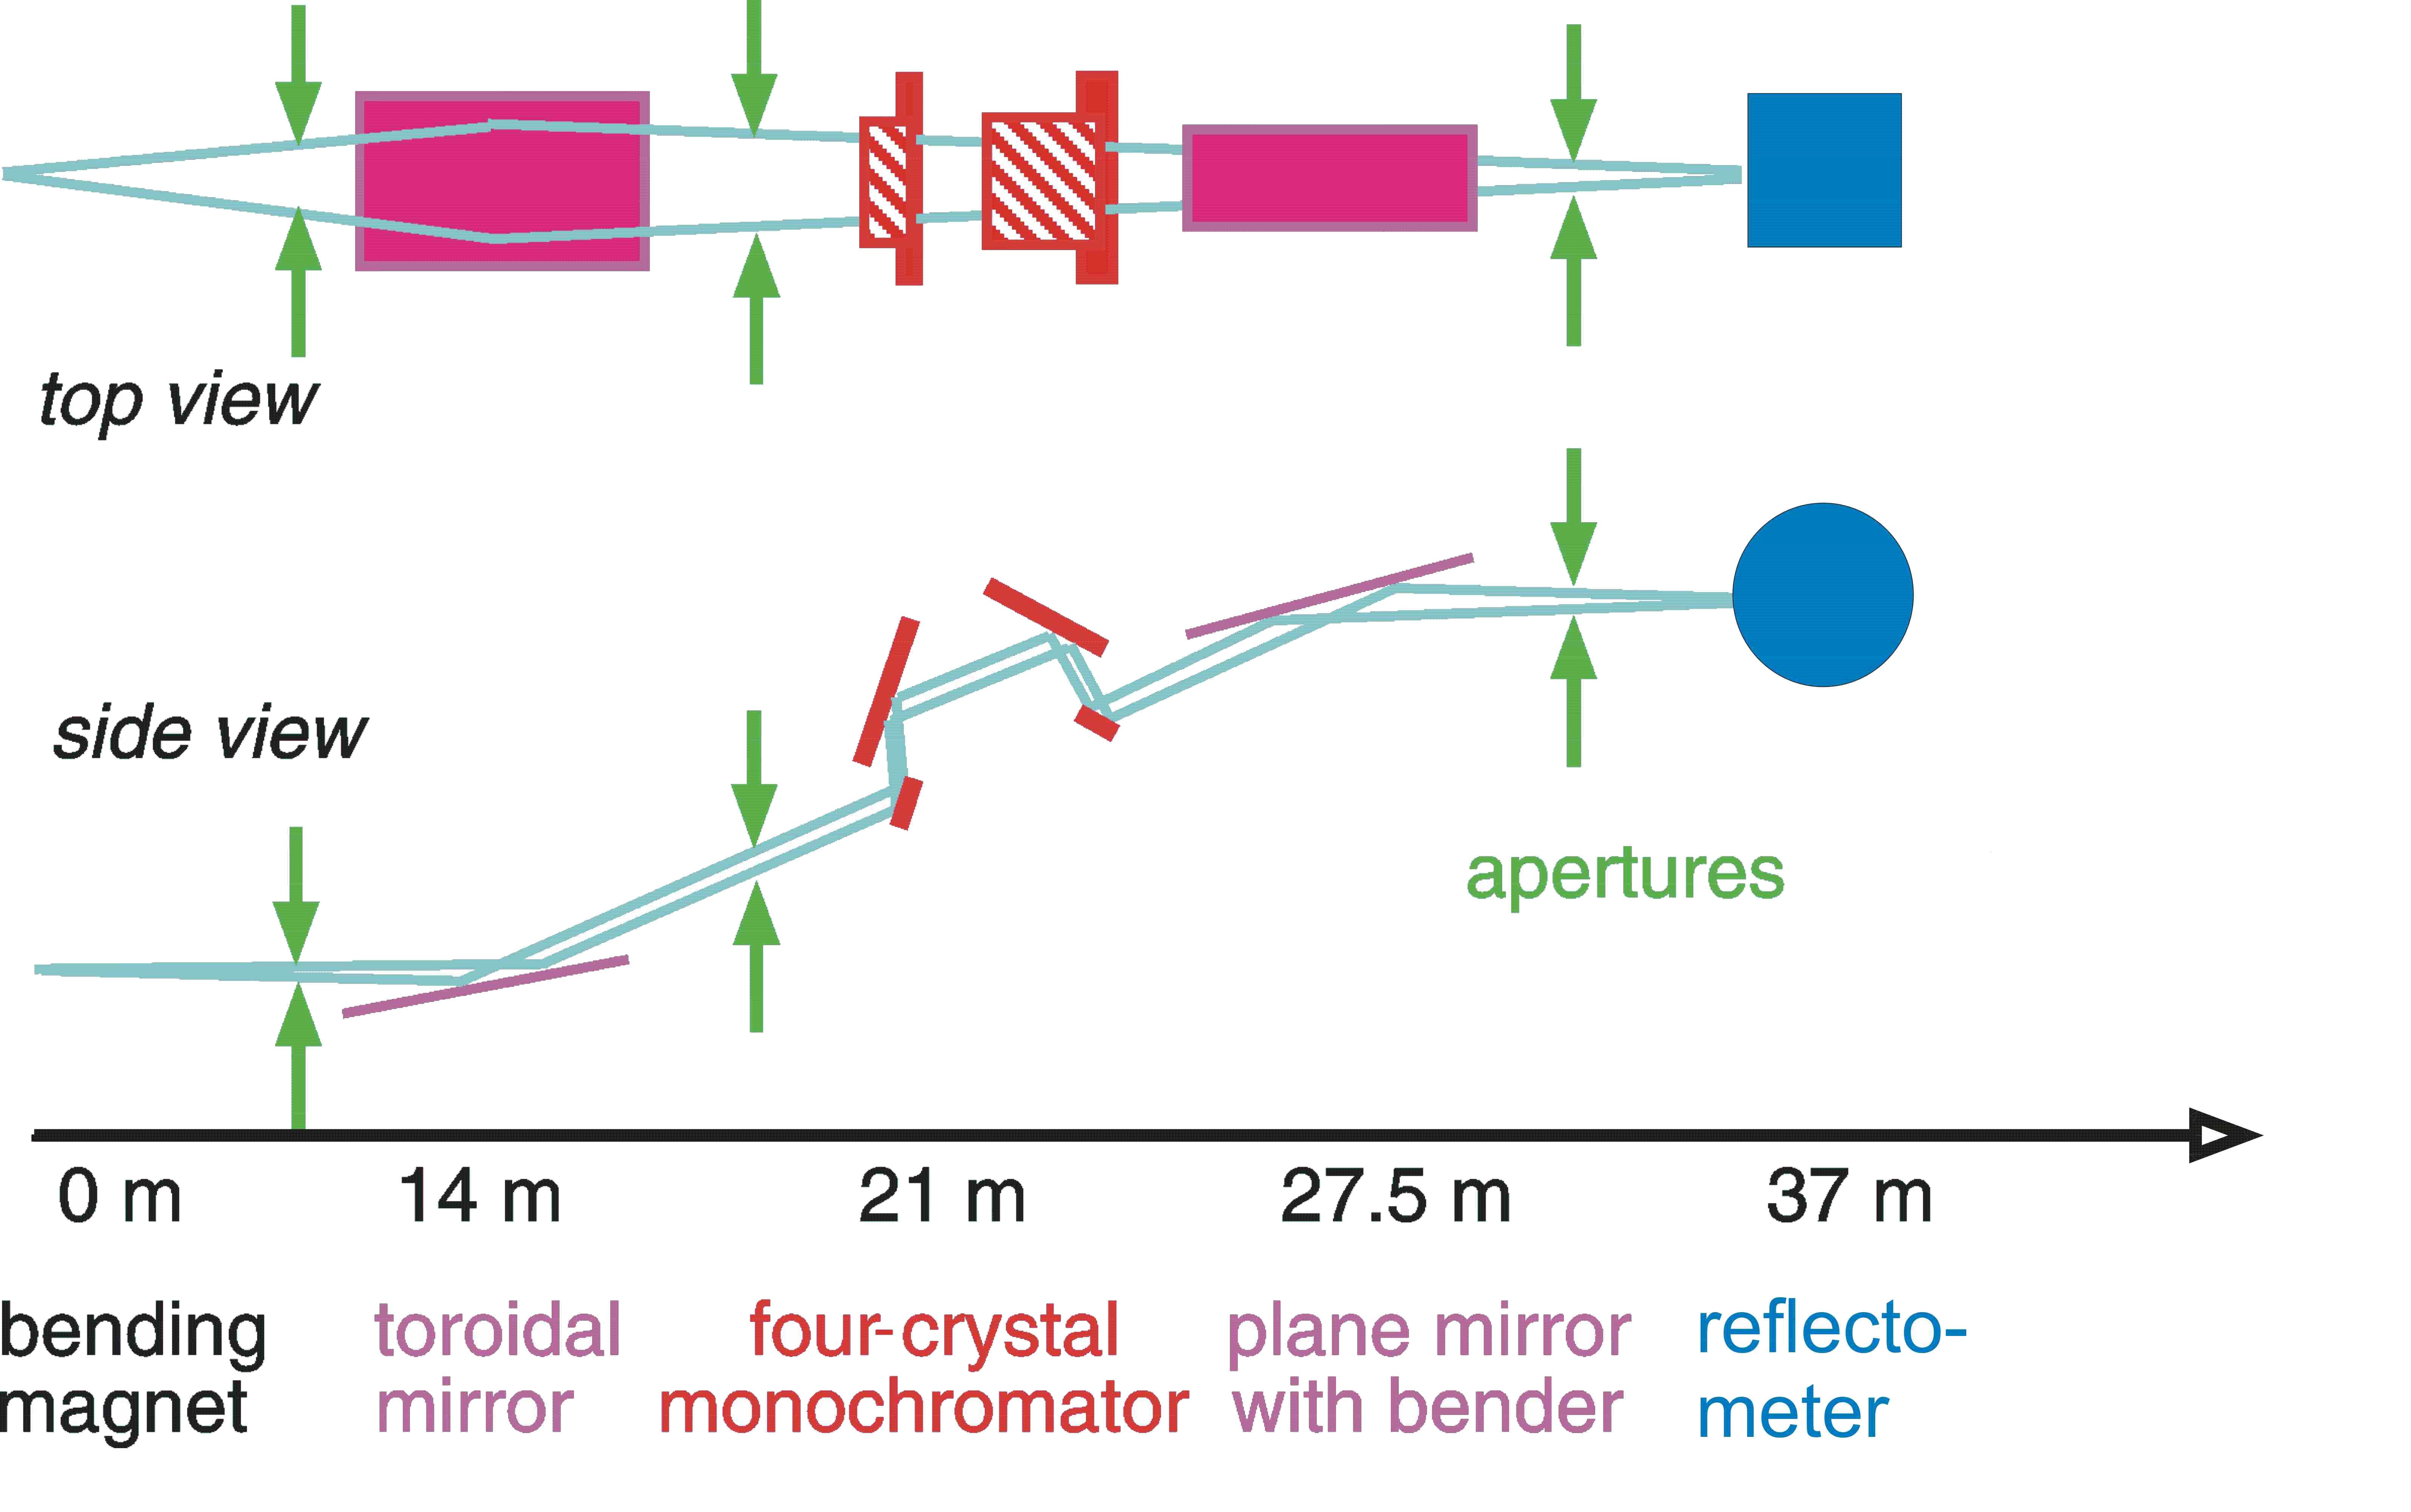
\includegraphics[width=0.7\textwidth]{img/FCMScheme.png}
        \caption[FCM beamline scheme.]{%
            FCM beamline scheme.}
        \label{ch_exp:fig_fcm_scheme}
\end{figure}

The end station used for the \gls{gixrf} experiments is a specialized chamber for \gls{gixrf}, \gls{txrf} and \gls{xrr} \cite{lubeck_novel_2013} depicted in Fig.~\ref{ch_exp:fig_gixrf_chamber}. It is equipped with a detector arm and a sample goniometer allowing to measure grazing incidence angles of \SI{0}{\degree} to \SI{60}{\degree}. The detector arm holds a diode allowing \gls{xrr} measurements. Perpendicular to the beam direction, an energy dispersive \gls{ssd} is mounted close to the sample surface. It allows to detect fluorescence radiation emitted from the sample energetically resolved. The samples can be rotated with respect to the storage ring plane in order to allow a variable polarization impinging on the surface.



\begin{figure*}[htb]
    \def\svgwidth{\textwidth}
    \import{svg/}{gixrf_chamber.pdf_tex}
    \caption[The GIXRF chamber.]{The GIXRF chamber.}
    \label{ch_exp:fig_gixrf_chamber}
\end{figure*}

\section{Sample systems}
The samples studied in the framework of this thesis are designed to work as near-normal incidence mirrors for the \gls{euv} spectral range. The underlying principle of an artificial one dimensional Bragg crystal requires the deposition of thin layered systems with high periodicity and stability. The experiments presented here were conducted on two sets of sample types as prototypes of mirrors for two different spectral ranges. The theoretical description of the principle of multilayer mirrors in Sec.~\ref{ch_theo:sec_multilayer} of Ch.~\ref{ch_theo}, optical contrast, i.e.~a large as possible difference in the real part of the refractive index $n$, is required to achieve large reflectivities, while on the other hand maintaining a low absorption.

This thesis investigates systems designed to reflect radiation in two spectral ranges, the \emph{water window} with wavelengths from \nm{2.2} to \nm{4.4} and the range from \nm{12.4} to \nm{14.0} with a wide range of applications, e.g.~for the next-generation lithography. The choice of the chemical species for the multilayer systems, apart from trivial properties such as non-toxicity and solidity, is largely influenced by the electronic structure of the respective materials, since large changes in the refractive index, i.e.~large optical contrast with respect to a second material, can be expected close to that resonances. The demand for low absorption also requires species, where the absorption edges are energetically higher or far lower than the desired spectral range of operation. For a well defined interface it is also neccessary that the two materials are mostly inert and do not react with one another. The latter would potentially lead to inevitable intermixing and thus a loss of a sharply defined interface.

\subsection{Choice of the Chemical Species and Multilayer Design}
\label{ch_exp:sec_multilayer_design}
\todo{mention spacer material and optically active material}

\paragraph{Cr/Sc multilayer system}
In case of the water window spectral range, we investigated samples designed for a peak reflectance at a wavelength closely above \nm{3.14}, where the L3 edge of scandium (Sc) is found. Fig.~\ref{ch_exp:fig_crsc_contrast} shows the refractive index of Sc and the second material chromium (Cr) in the water window spectral range. 
\begin{figure}[htb]
        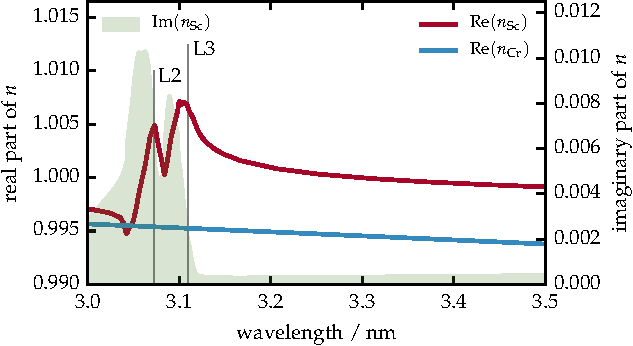
\includegraphics{img/Cr_Sc_contrast}
        \caption[Refractive indices of Cr and Sc in the water window.]{%
            Refractive indices of Cr and Sc with the water window spectral range. The marked absorption edges are the L2 and L3 edge of Sc. The imaginary part of the refractive index accounts for the absorption and is shown for Sc. Above the L3 edge is the highest contrast for the two materials providing the highest potential reflectivity in a periodic multilayer arrangement.}
        \label{ch_exp:fig_crsc_contrast}
\end{figure}
The periodic multilayer of the systems investigated here, were therefore binary alternating layers of Cr and Sc. The required nominal period thickness $D$, i.e.~the thickness each periodically repeated layer stack, for the design goal of a peak reflectivity at $\lambda=\nm{3.14}$ is $D=\nm{1.573}$ with a layer thickness ratio of $\Gamma=0.5$ of both materials. To protect the Sc layers from oxidation, an additional capping layer Cr of approximately $d_\text{cap} = \nm{3}$ was added as the surface layer. The binary layer stack was repeated $N=400$ times per bilayer.

The Cr/Sc multilayer sample was prepared at the DESY X-ray multilayer 
laboratory by DC magnetron sputtering. The deposition was performed at $0.133$ 
Pa ultrahigh purity Ar ($99.999\%$) and a power of $200$ W for both Sc and Cr 
sputtering targets. The multilayer is composed of alternating layers of Cr and 
Sc with periodic replication of the bilayer stack by $N=400$ times. The 
substrate is a superpolished Si wafer piece. The sample dimensions measure 
approximately $(20 \times 20)$ mm$^2$. More details can be found elsewhere 
\cite{prasciolu_thermal_2014}. The multilayer mirror was designed to reflect 
radiation in the water window energetically, just below the Sc L edge, close to 
a $3.1$ nm wavelength at an angle of incidence (AOI) of $\alpha_i = 
88.5^\circ$.


\paragraph{Mo/Si multilayer systems}
The second set of systems under investigation in this thesis is composed out of $50$ to $65$ bilayers Molymdenum (Mo) and Silicon (Si). Both materials show a very low absorption in the range from \nm{12.4} to \nm{14.0}, with the Si L2 edge forming the lower wavelength limit for the usage as a mirror system in this combination. The respective refractive indices are given in Fig.~\ref{ch_exp:fig_mosi_contrast}.
\begin{figure}[htb]
        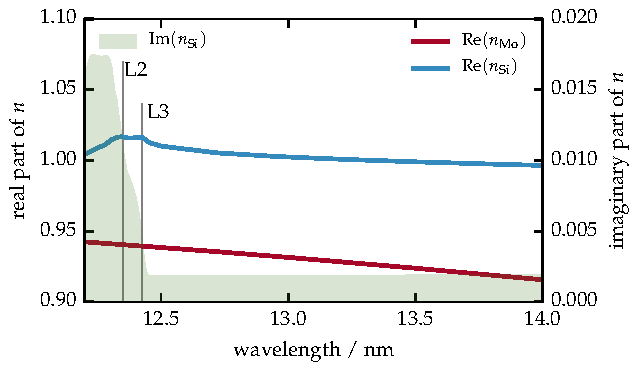
\includegraphics{img/Mo_Si_contrast}
        \caption[Refractive indices of Mo and Si in the wavelength range from \nm{12.4} to \nm{14.0}.]{%
            Refractive indices of Mo and Si in the wavelength range from \nm{12.4} to \nm{14.0}. The L2 absorption edge of Si marks the lower wavelength limit for the applicability of this material combination in multilayer mirror systems.}
        \label{ch_exp:fig_mosi_contrast}
\end{figure}

Finally, the sample systems can contain additional materials, which serve as barrier layers. The two species used for our samples are Boroncarbite (B$_4$C) and Carbon (C). Those two materials do not have any absorption edges in the given relevant spectral range and additionally show low contrast to the respective spacer materials Si and Cr. The details of the respective sample layouts are discussed in the respective sections of the following chapters.

\subsection{Multilayer Deposition by Magnetron Sputtering} \label{ch_exp:sec_magnetron_sputtering}
The multilayer samples investigated here were fabricated by the DC magnetron sputtering technique \cite{stearns_fabrication_1991} by two different multilayer and optics groups. The Mo/Si multilayer samples were fabricated by Stefan Braun at the Fraunhofer IWS, Dresden, Germany and the Cr/Sc samples are by Sa\v{s}a Bajt from the Optics Group at CFEL, DESY, Hamburg in Germany.

Magnetron sputtering is a physical vapor deposition technique. A vacuum chamber is equipped with a substrate to be coated, in our case silicon, and one or more sputter targets. Depending on the intended design of the multilayer to be deposited, those targets are the respective materials, which later form the individual layers. In the DC magnetron sputtering system, a strong electric field is applied between the substrate and the sputter targets. The vacuum chamber containing those parts is then filled with a sputter gas, typically ultrapure Ar gas (\SI{99.999}{\percent}), with partial pressures in the range from \mbar{E-3} to \mbar{E-2} \cite{stearns_fabrication_1991}. The strong electric field ionizes the sputter gas causing the ions to be accelerated towards the sputter targets (cathode) and form a charged plasma. Upon impact in the target, atoms and electrons of the condensed matter phase of the respective material are released and travel towards the substrate. The released atoms condense there, forming bonds and creating a slowly growing layer. The thickness of the layer can be fine tuned through the deposition time. The additionally released electrons, while being accelerated towards the substrate (anode), collide with the sputter gas atoms and cause further ionization. In order to avoid damage of the forming layer at the substrate, strong magnetic fields are applied to the sputter targets. This confines the movement of the charged particles (the plasma) sputter gas ions and electrons to the region close to the target surface. Thereby, increasing the collision (ionization) probability of electrons and the gas atoms through the helical movement in the magnetic field while keeping those particles away from the substrate. To ensure homogeneous layer deposition, the substrate is kept under permanent rotation. A schematic DC magnetron sputtering system is depicted in Fig.~\ref{ch_exp:magnetron_sputtering_schematic}.
\begin{figure}[htb]
        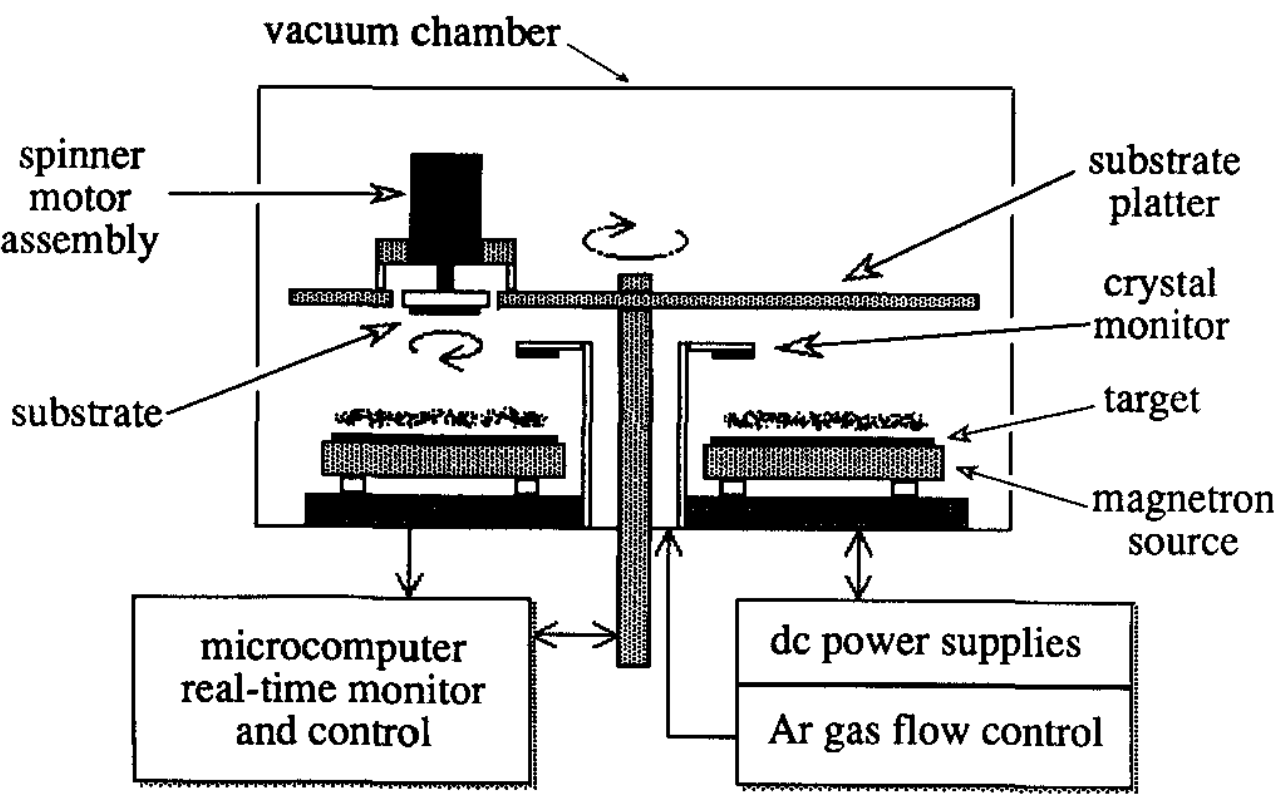
\includegraphics[width=0.7\textwidth]{img/magnetron_sputtering_schematic.png}
        \caption[Schematic setup for magnetron sputtering.]{%
            Schematic setup for magnetron sputtering.}
        \label{ch_exp:magnetron_sputtering_schematic}
\end{figure}


For both samples, silicon serves as the substrates for the deposition process. The surfaces are super polished with mechanical polishing methods to reduce any prior surface roughness. The sample size and shape differ for the systems investigated. In case of the Mo/Si mirror samples, wafer pieces of approximately $\mm{20} \times \mm{20}$ (photograph shown in Fig.~\ref{ch_exp:fig_mosi_sample}) and round substrates with approximately \mm{20} in diameter were used.
\begin{figure}[htb]
        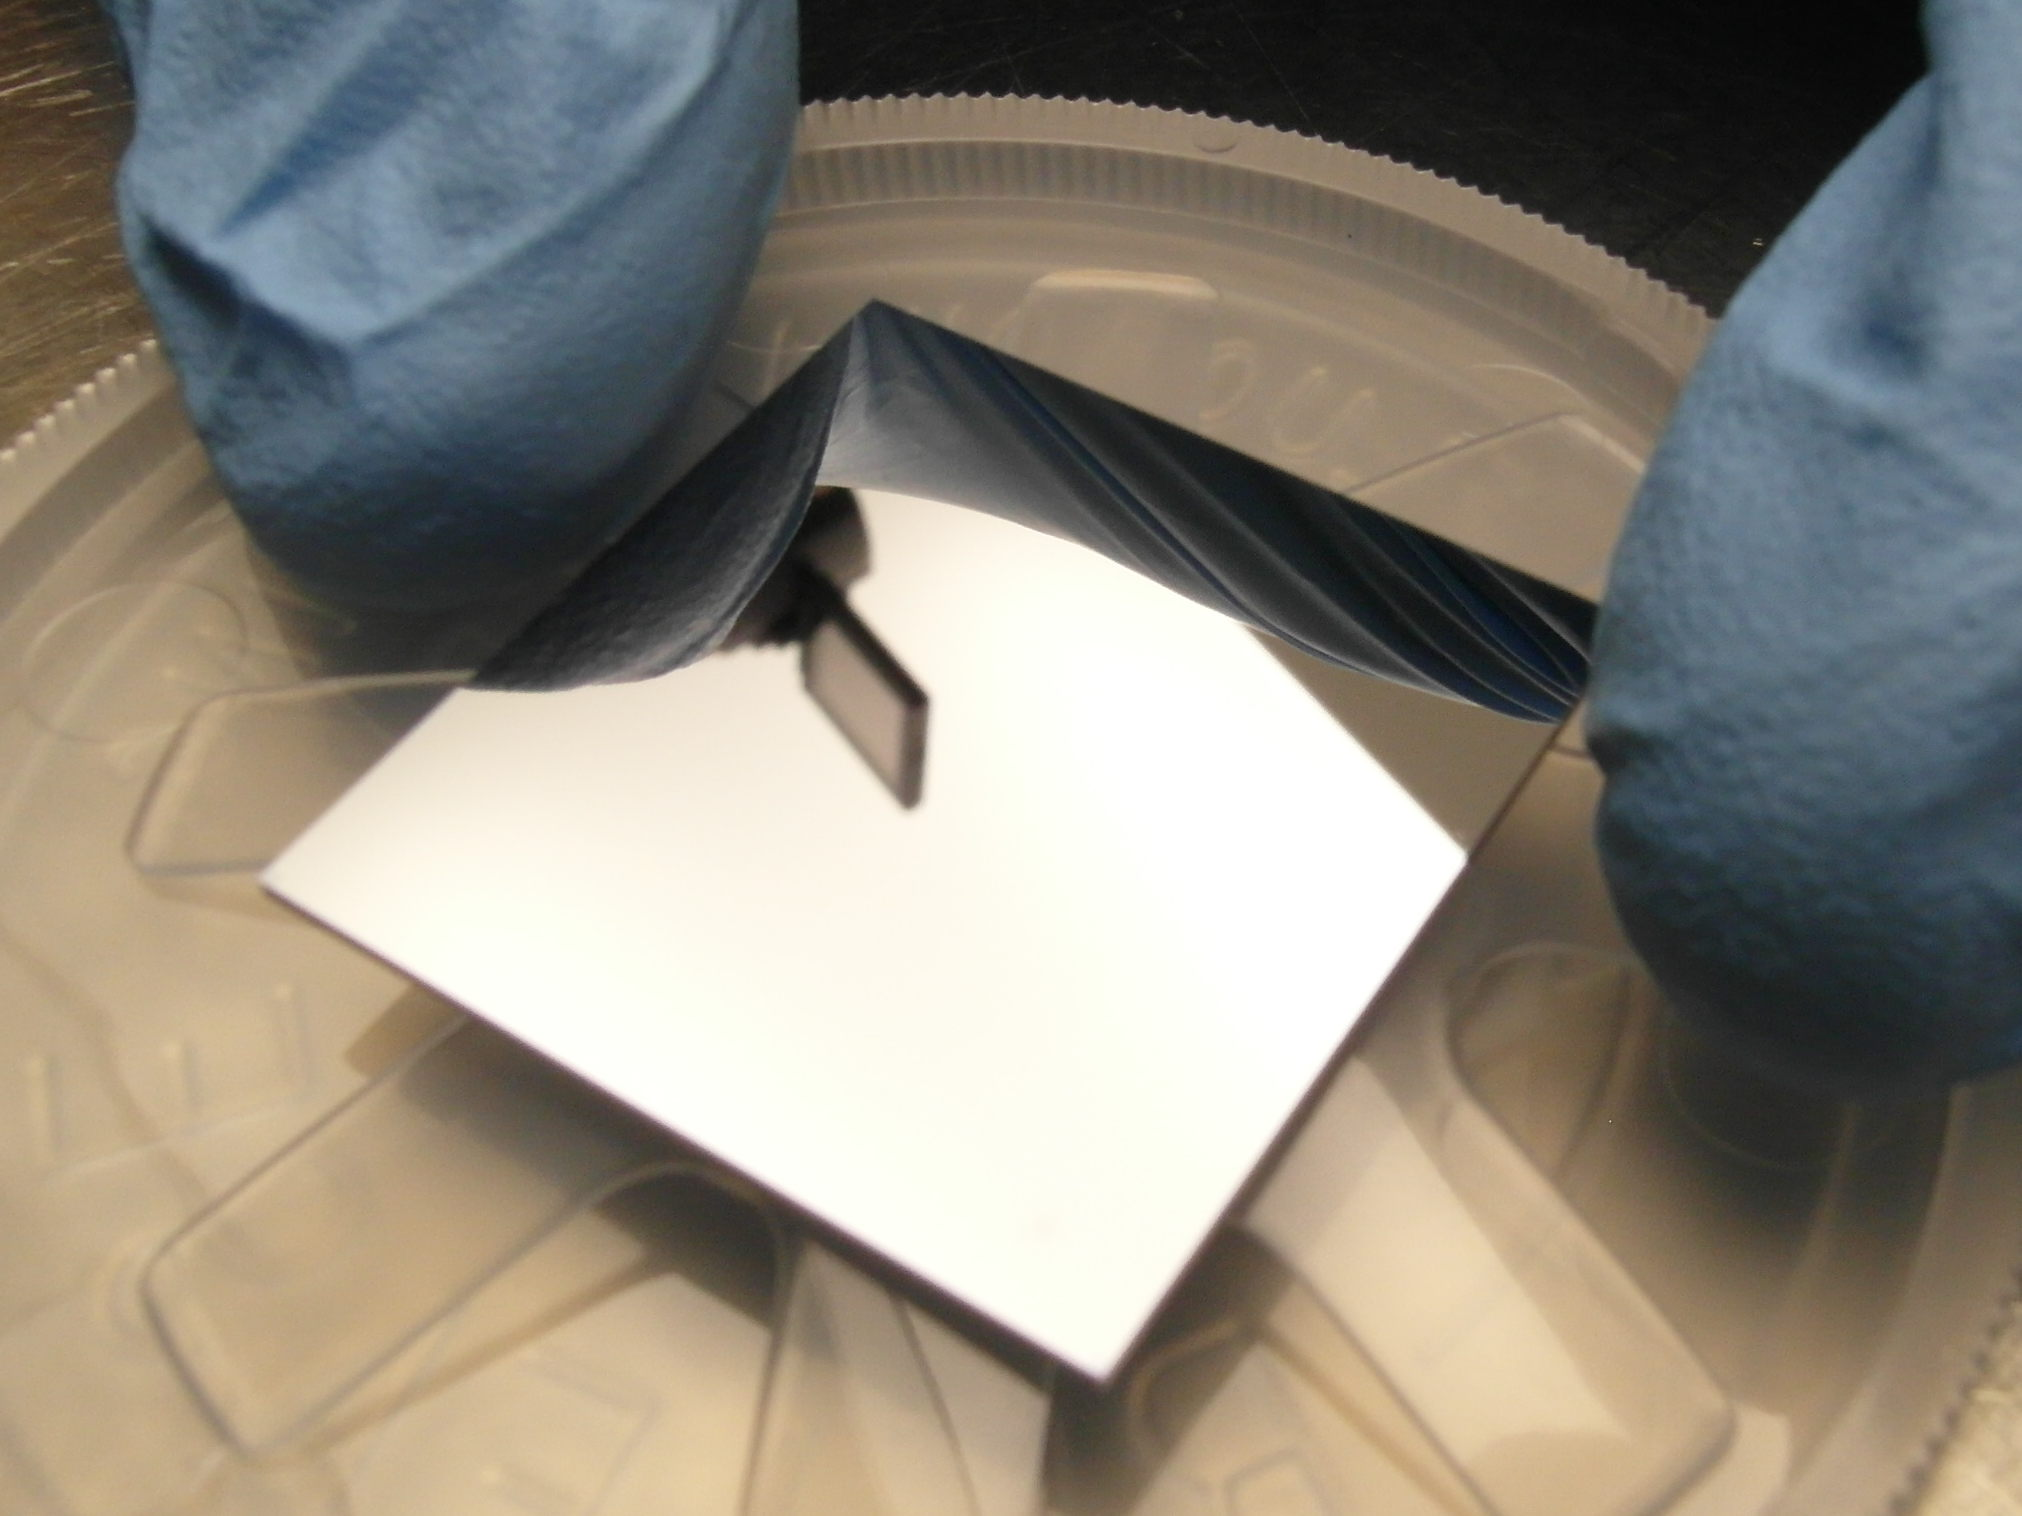
\includegraphics[width=0.4\textwidth]{img/SAM_1910_v1}
        \caption[Mo/Si multilayer sample.]{%
            Mo/Si multilayer sample.}
        \label{ch_exp:fig_mosi_sample}
\end{figure}
In case of the Cr/Sc systems, wafer pieces of varying size but approximately $\mm{10} \times \mm{20}$ served as the substrate.
